\documentclass[12pt]{article}

\usepackage[margin=0.5in]{geometry}
\usepackage{hyperref}
\hypersetup{
    colorlinks=true,
    linkcolor=blue,
    filecolor=magenta,      
    urlcolor=cyan,
    pdftitle={Overleaf Example},
    pdfpagemode=FullScreen,
    }
\urlstyle{same}
\usepackage{graphicx}
\usepackage{listings}
\usepackage{xcolor}

\definecolor{codegreen}{rgb}{0,0.6,0}
\definecolor{codegray}{rgb}{0.5,0.5,0.5}
\definecolor{codepurple}{rgb}{0.58,0,0.82}
\definecolor{backcolour}{rgb}{0.95,0.95,0.92}

\lstdefinestyle{mystyle}{
    backgroundcolor=\color{backcolour},   
    commentstyle=\color{codegreen},
    keywordstyle=\color{magenta},
    numberstyle=\tiny\color{codegray},
    stringstyle=\color{codepurple},
    basicstyle=\ttfamily\footnotesize,
    breakatwhitespace=false,         
    breaklines=true,                 
    captionpos=b,                    
    keepspaces=true,                 
    numbers=left,                    
    numbersep=5pt,                  
    showspaces=false,                
    showstringspaces=false,
    showtabs=false,                  
    tabsize=2
}


\lstset{style=mystyle}
\usepackage{}

\title{Introduction to modelling and programming}
\author{Nathan Hughes}
\date{\today}


\begin{document}
\maketitle

\section{Setup}


In this session we will be using the Python programming language. To avoid having to install anything, and for a quick start, we will be using \url{https://colab.research.google.com/}. Colaboratory is a service offered by Google that allows running Python (and some other languages) code remotely. If you're interested in continuing with anything covered in this session then \href{https://www.anaconda.com}{Anaconda} is a very simple, user-friendly, method of installing Python onto your own computer. 

\textbf{Before this session}, please ensure that you can do the following: 

\begin{enumerate}
    \item Go to \url{https://colab.research.google.com/} and sign-in (can use your own Google account or create a new one if needed).
    \item Go to file $\rightarrow$ new notebook.
    \item You'll now see an empty file, there will be a blank box. Into this box type "print('hello world!')".
    \item Press the run button and check that it properly prints out your message. 
\end{enumerate}

\begin{figure}[!h]
    \centering
    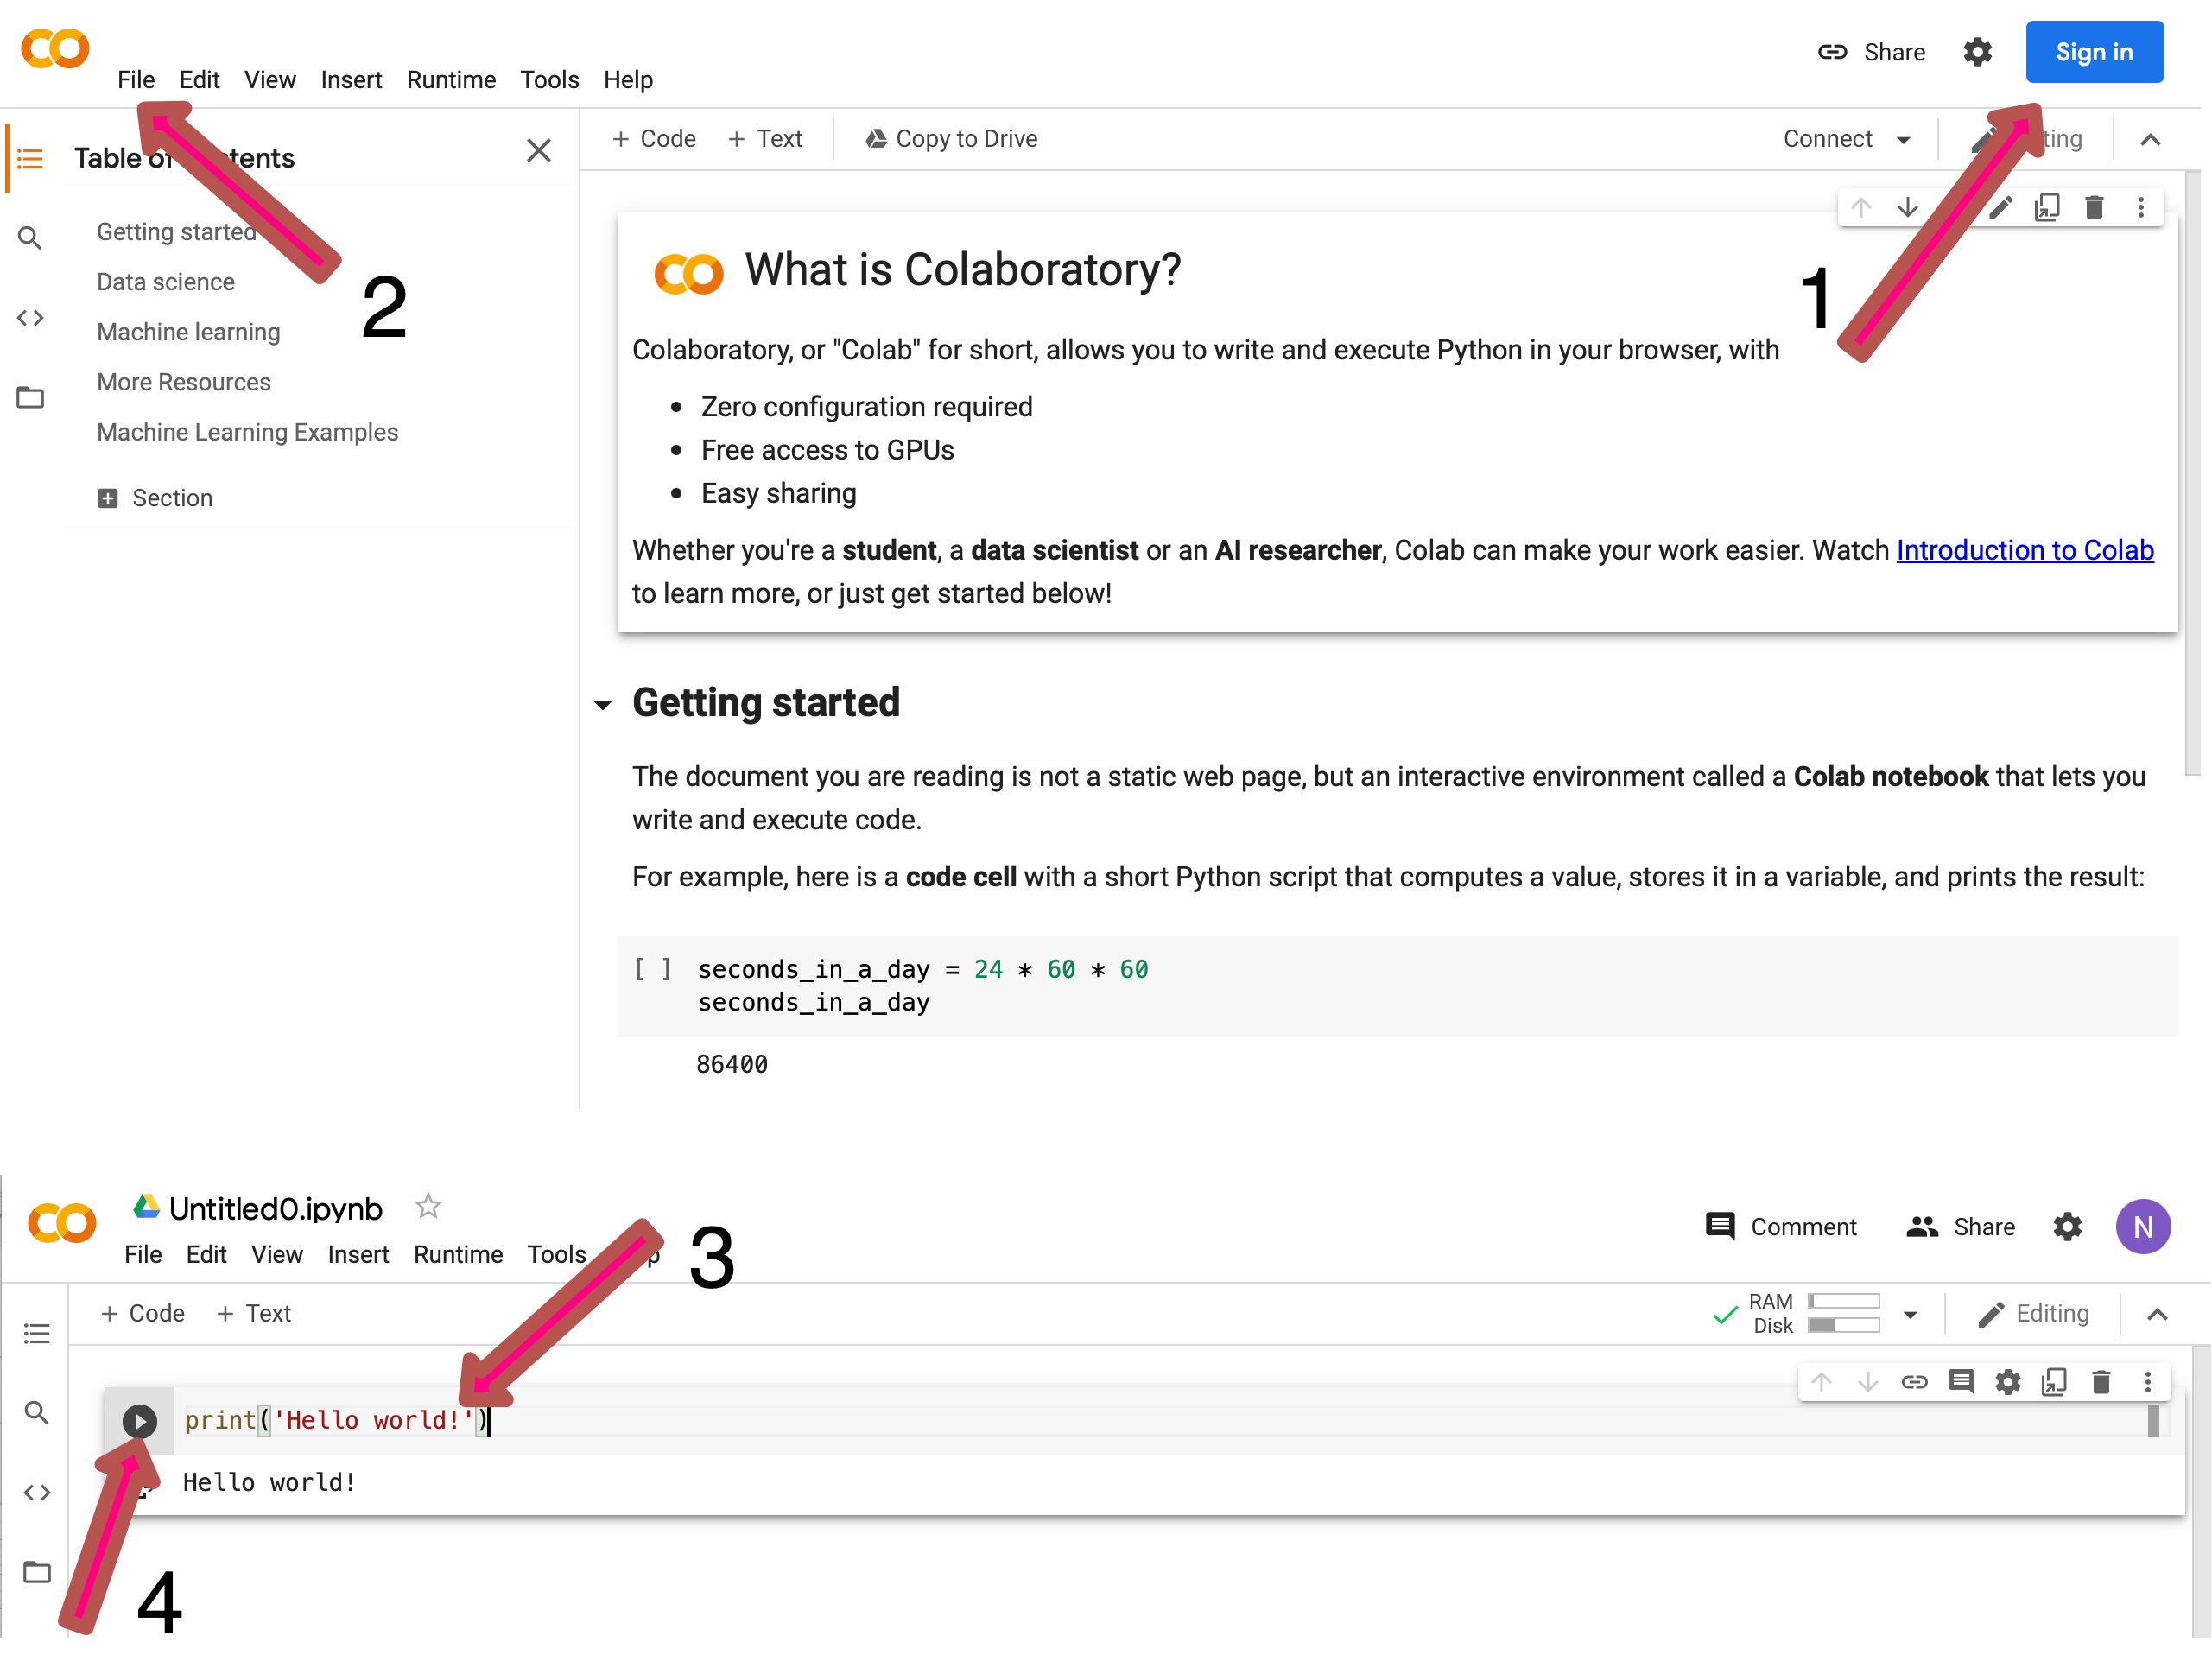
\includegraphics[width=0.6\textwidth]{./figures/ssIM1.png}
    \caption{Getting setup on Google Colaboratory}
\end{figure}


\section{Introduction to Python}

Python is an example of an "interpretive" programming language. This means that it runs exactly what it's told to, when it's told to. This makes it ideal for modelling and exploring data as we do not need to plan out exactly what we want to do with the data as we are working with it. 

Before we begin with using data and doing any modelling, we must first learn some basics of how to use Python.

\subsection{Basic mathematics operations}

If we followed the setup section properly we will have what is called a "Python Notebook" in front of us. This allows us to type some code into a box then hitting run to get some results. Starting off simple we can delete anything which was previously in the box and type some basic maths operations such as: 

Addition:
\begin{lstlisting}[language=Python]
    1+1
\end{lstlisting}

Subtraction:
\begin{lstlisting}[language=Python]
    1-1-1-1
\end{lstlisting}

Multiplication and division:
\begin{lstlisting}[language=Python]
    10*10/5
\end{lstlisting}

Powers:
\begin{lstlisting}[language=Python]
    10**2
\end{lstlisting}

Also, please notice that order of operations matter, just like in maths. If you want to specify operations you can always add "()". 

\subsection{Variables}

In most programming languages it is important to consider what kind of data you are using e.g. is it text, integer values, floating point values, etc. Python is pretty smart and lets you move between these types vary easily and without specifying explicitly what you want. For example we can make a named variable like so: 


\begin{lstlisting}[language=Python]
    i = 10
\end{lstlisting}

Then do some operations on it: 


\begin{lstlisting}[language=Python]
    i + 5
\end{lstlisting}

Or even change it and check it again (notice what happens, and is it what you expected to happen?): 

\begin{lstlisting}[language=Python]
    i = i + i 
    print(i)
\end{lstlisting}

Using variables makes it easier to generalise code: 

\begin{lstlisting}[language=Python]
    x = 5
    y = 10
    z = 20

    volume = x * y * z
    print(volume)
\end{lstlisting}

\subsection{Making and using functions}

The real power of programming solutions is really the ability to create reproducible results. As scientists, it is critical that our code always give the same results when given the same input.  In Python, we can create functions which allow us to make code reusable and to save copying and pasting and possibly making mistakes. To create a function we use the word "def" followed by whatever name we want to use, some "()" which will include the parameters of the function, a ":" and then under all that the actual function itself.

\begin{lstlisting}[language=Python]
    def myFirstFunction(a):
        return a*2
\end{lstlisting}

With this example we created a function called "myFirstFunction" which takes one parameter "a" and returns a value twice that of "a". Notice that running a block with this code will not do anything. That's because we haven't actually used it.  This is exactly the same as $f(a) = 2a$, if you want to think of it more mathematically.

To use this function we need to call it, so creating a new code box with the "+" button we can now try: 

\begin{lstlisting}[language=Python]
myFirstFunction(5)
\end{lstlisting}

You may have noticed by calling "myFirstFunction" looks similar to the "print(x)" command, and it is, they're both functions in python. 

We can use functions within functions to make more complicaticated behaviours: 

\begin{lstlisting}[language=Python]

    def volumeOfCuboid(x,y,z):
        print("X is equal to", x)
        print("Y is equal to", y)
        print("Z is equal to", z)
        print("----")
        volume = x*y*z
        print("Volume is":)
        print(volume)
        return volume

    volumeOfCuboid(10,20,30)
    
    a = 5
    b = 10
    c = 2

    volumeOfCuboid(a,b,c)
\end{lstlisting}
    
\subsection{Lists, dictionaries and Loops}

So far we have used small variables such as $x=10$, but often we want to work with a series of values such as $X = [1,2,3,4,5]$. In Python the basic way to do this is with "lists", in the next section we will talk about "arrays", take note that there is a difference. 

We can make a basic list like this:

\begin{lstlisting}[language=Python]

    myShoppingList = ['milk', 'bread', 'tofu']
    print(myShoppingList)
\end{lstlisting}

and also add to the list like this, using the ".append" function:

\begin{lstlisting}[language=Python]
    myShoppingList = ['milk', 'bread', 'tofu']
    print(myShoppingList)
    print('Opps I forgot to add apples')
    myShoppingList.append('apples')
    print(myShoppingList)
\end{lstlisting}

Lists are ordered and indexed, meaning we can access just a selection if we want:

\begin{lstlisting}[language=Python]
    myShoppingList = ['milk', 'bread', 'tofu']

    print("the first thing in my list is")
    print(myShoppingList[0])

\end{lstlisting}

Notice that we begin counting the list at "0" and not "1". 

Python also makes it very easy to loop over lists. Look at the following code and think what it's doing. The value "i" can be anything, I just named it 'i" for an example. Also, notice the indentation of the list:

\begin{lstlisting}[language=Python]
    myShoppingList = ['milk', 'bread', 'tofu']

    for i in myShoppingList:
        print(i)

\end{lstlisting}

Another kind of list-like structure in Python is a "dictionary". It is somewhat similar to a list only it doesn't have to be numbers indexing it. For example: 

\begin{lstlisting}[language=Python]
    Ages = {"Ben" : 10, "Spider-man": 34, "Claire": 24}
    print(Ages["Ben"])
\end{lstlisting}

Adding to dictionaries is a little different too:

\begin{lstlisting}[language=Python]
    Ages = {"Ben" : 10, "Spider-man": 34, "Claire": 24}

    print("ahh, we forgot to get Tom's age")
    Ages['Tom'] = 17

    print(Ages)
\end{lstlisting}

\subsection{Importing libraries Numpy and Matplotlib}

One of the most commonly used libraries in Python is called "numpy" it allows for some pretty cool mathematical functionality. To import a library (if you're running this on your own computer you may need to install first, but on Colaboratory it should already be installed). 

For example, if we want a function to square root a number we can first import the numpy library and then do a "." to access its 'sqrt" function. The "." basically can be thought of as saying "within", so "within numpy" use "sqrt". 

\begin{lstlisting}[language=Python]
    import numpy 

    i = 100 
    numpy.sqrt(i)
\end{lstlisting}

We use numpy a lot, so to make it a little shorter to type we can change this to use an alias of "np". Look how this example is different:

\begin{lstlisting}[language=Python]
    import numpy as np 

    i = 100 
    np.sqrt(i)
\end{lstlisting}

With numpy we can work with what is called an array, these a similar to matricies in mathematics, but can be N-dimensional. For example a 1-D array we can make like this:

\begin{lstlisting}[language=Python]
    myArray = np.arange(1,10)
    print(myArray)
\end{lstlisting}

Now with numpy we can quickly generate some arrays we may want to stop looking at just text and think about it in plots and figures using matplotlib:

\begin{lstlisting}[language=Python]
    import matplotlib.pyplot as plt 
    import numpy as np 

    Xs = np.arange(0,10)
    sin_values = []
    for v in Xs:
        sin_values.append(np.sin(v))

    plt.plot(Xs, sin_values)

\end{lstlisting}

\textbf{Stop here:} we've just put together a lot of things, and it's very important at this point that we look at each line and ensure we know what it's doing. You don't have to understand perfectly, but realise what each line is adding and why it is needed.

So, if you've got this plot to work you may think it looks a little clunky, let's do a few things to tidy it up:

\begin{lstlisting}[language=Python]
    import matplotlib.pyplot as plt 
    import numpy as np 

    sin_values = []
    Xs = np.linspace(0,10, num=1000)
    for x in Xs:
        sin_values.append(np.sin(x))
    plt.plot(Xs, sin_values)
    plt.xlabel('x')
    plt.ylabel('sin(x)')
    plt.grid()

\end{lstlisting}

Once again, look at what we've added and changed. The new function of "np.linspace", try Googling this and see if you can read and understand what this function does. 


\subsection{Testing your knowledge}

Before we move onto actually modelling here is a short challenge which you should be able to do with a little bit of thought and maybe a small Google search. 

You must make a new plot, on this plot you will first plot $2 \times \sin(x)$ values for 0 to 100 and then on the same figure plot the values of $\sqrt[3]{\sin(x)}$ for the same range. Bonus points if you can add a label to these lines. An example solution can be found at the back of this booklet. 

\begin{figure}[!h]
    \centering
    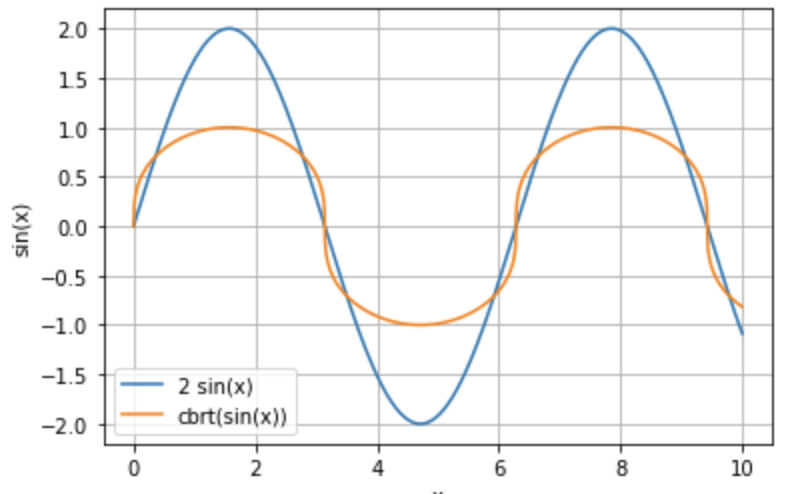
\includegraphics[width=0.6\textwidth]{figures/ssIM3.png}
    \caption{How your figure should look if you can complete this test}
\end{figure}

\subsection{Bonus round: can you debug this}

Here are some examples of almost working code, can you tell what is wrong and fix it so that it works? 


\begin{lstlisting}[language=Python]
    X = 
    print(X)
\end{lstlisting}


\begin{lstlisting}[language=Python]
    X = 10
    print(X
\end{lstlisting}


\begin{lstlisting}[language=Python]
    def f(x):
        print(y)

    f(10)
\end{lstlisting}

\begin{lstlisting}[language=Python]
    a = "a"
    b = 6

    a+b
\end{lstlisting}

\clearpage

\section{The Iris dataset}

The \href{https://en.wikipedia.org/wiki/Iris_flower_data_set}{Iris data set} is a multivariate data set introduced by Ronald Fisher. It consists of measurements of sepal length, sepal width, petal length and petal width for three species of Iris plants, \textit{Iris setosa, Iris versicolor} and \textit{Iris Virginica}. This data set contains 50 measurements for each species and is often used for data science / modelling examples. 

\begin{figure}[!h]
    \centering
    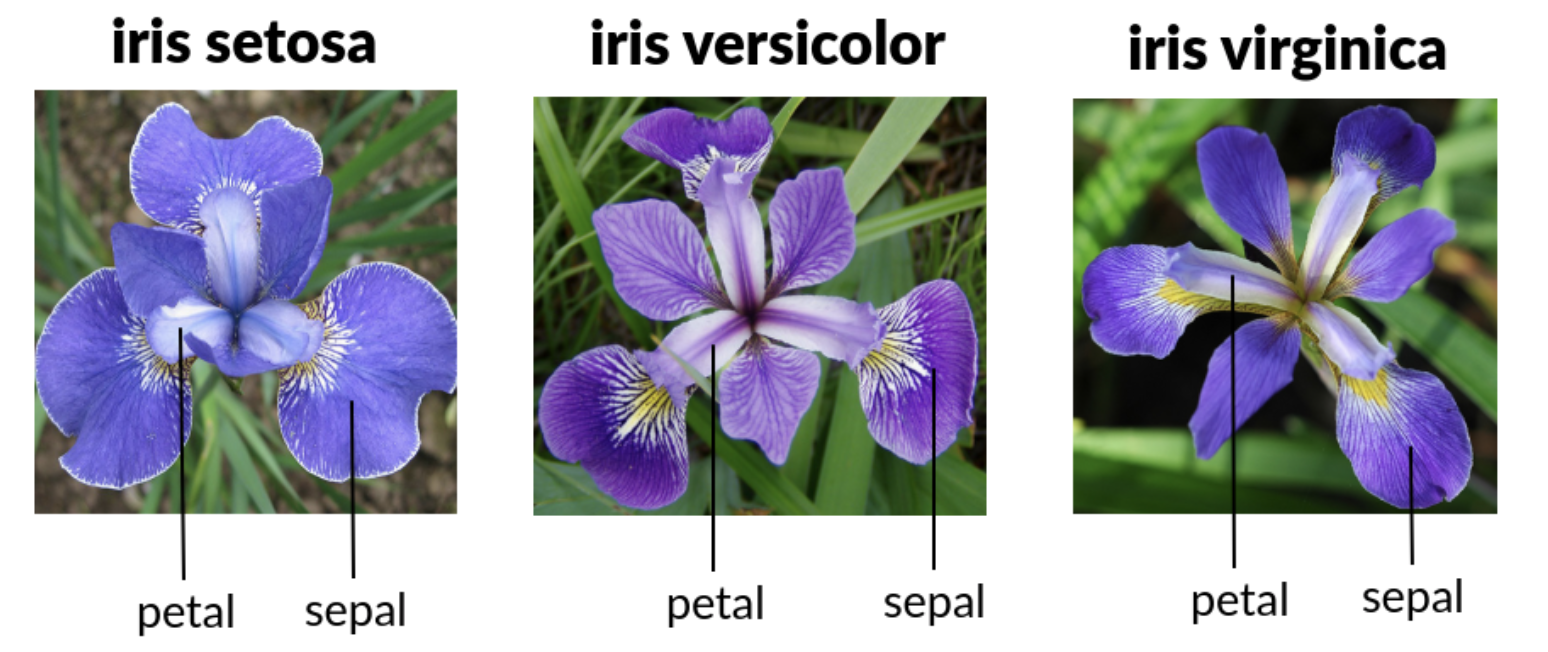
\includegraphics[width=0.7\textwidth]{figures/ssIM2.png}
    \caption{Example of each Iris species used in the Iris data set}
\end{figure}

\subsection{Loading and exploring data} 

Again, speed and efficency of our time, is the name of the game here so we're going to introduce two new libraries to help us get our hands on this data set and explore it: 

\begin{lstlisting}[language=Python]
    import seaborn as sns 
    import pandas as pd

    df=sns.load_dataset('iris')
    df.head()
\end{lstlisting}

Seaborn is a package which makes matplotlib a little quicker to use, and pandas is a beautiful little library for working with tables of data. We call these tables "Dataframes" which is why we abbreviate the data to "df" for quickness. Calling the ".head()" function on the Dataframe gives us a quick look at the first few rows of data. 

\begin{table}[!h]
    \centering
    \begin{tabular}{crrrrr}
    \multicolumn{1}{r}{\textbf{}} & \textbf{sepal\_length} & \textbf{sepal\_width} & \textbf{petal\_length} & \textbf{petal\_width} & \textbf{species} \\
    \textbf{0}                    & 5.1                    & 3.5                   & 1.4                    & 0.2                   & setosa           \\
    \textbf{1}                    & 4.9                    & 3.0                   & 1.4                    & 0.2                   & setosa           \\
    \textbf{2}                    & 4.7                    & 3.2                   & 1.3                    & 0.2                   & setosa           \\
    \textbf{3}                    & 4.6                    & 3.1                   & 1.5                    & 0.2                   & setosa           \\
    \textbf{4}                    & 5.0                    & 3.6                   & 1.4                    & 0.2                   & setosa          
    \end{tabular}
    \end{table}

With these data and pandas we can do some very quick and very useful analysis. For example, if we want to check the mean of all columns:
\begin{lstlisting}[language=Python]
    df.mean()
\end{lstlisting}

% Or, being more specific the mean of each species:
% \begin{lstlisting}[language=Python]
%     df.groupby('species').mean()
% \end{lstlisting}

% \begin{table}[!h]
%     \centering
%     \begin{tabular}{crrrrr}
%     \multicolumn{1}{r}{\textbf{}}        & \textbf{sepal\_length} & \textbf{sepal\_width} & \textbf{petal\_length} & \textbf{petal\_width} & \textbf{} \\
%     \multicolumn{1}{r}{\textbf{species}} & \textbf{}              & \textbf{}             & \textbf{}              & \textbf{}             &           \\
%     \textbf{setosa}                      & 5.006                  & 3.428                 & 1.462                  & 0.246                 &           \\
%     \textbf{versicolor}                  & 5.936                  & 2.770                 & 4.260                  & 1.326                 &           \\
%     \textbf{virginica}                   & 6.588                  & 2.974                 & 5.552                  & 2.026                 &               \end{tabular}
% \end{table}

Alternatively, we can use another handy function called "describe" like so:

\begin{lstlisting}[language=Python]
    df.describe()
\end{lstlisting}

\begin{table}[!h]
    \centering
    \begin{tabular}{crrrrr}
    \multicolumn{1}{r}{\textbf{}}      & \textbf{sepal\_length} & \textbf{sepal\_width} & \textbf{petal\_length} & \textbf{petal\_width} & \textbf{}            \\
    \multicolumn{1}{r}{\textbf{count}} & 150.000000             & 150.000000            & 150.000000             & 150.000000            &                      \\
    \textbf{mean}                      & 5.843333               & 3.057333              & 3.758000               & 1.199333              &                      \\
    \textbf{std}                       & 0.828066               & 0.435866              & 1.765298               & 0.762238              &                      \\
    \textbf{min}                       & 4.300000               & 2.000000              & 1.000000               & 0.100000              &                      \\
    \textbf{25\%}                      & 5.100000               & 2.800000              & 1.600000               & 0.300000              &                      \\
    \multicolumn{1}{l}{\textbf{50\%}}  & 5.800000               & 3.000000              & 4.350000               & 1.300000              & \multicolumn{1}{l}{} \\
    \multicolumn{1}{l}{\textbf{75\%}}  & 6.400000               & 3.300000              & 5.100000               & 1.800000              & \multicolumn{1}{l}{} \\
    \multicolumn{1}{l}{\textbf{max}}   & 7.900000               & 4.400000              & 6.900000               & 2.500000              & \multicolumn{1}{l}{}
    \end{tabular}
    \end{table}

\subsection{Plotting data}
This is nice and all, but what about making some nicer summary plots, boxplots for example, are a nice way to show distributions:

\begin{lstlisting}[language=Python]
    sns.boxplot(data=df, x='species', y='petal_width')
\end{lstlisting}

\begin{figure}[!h]
    \centering
    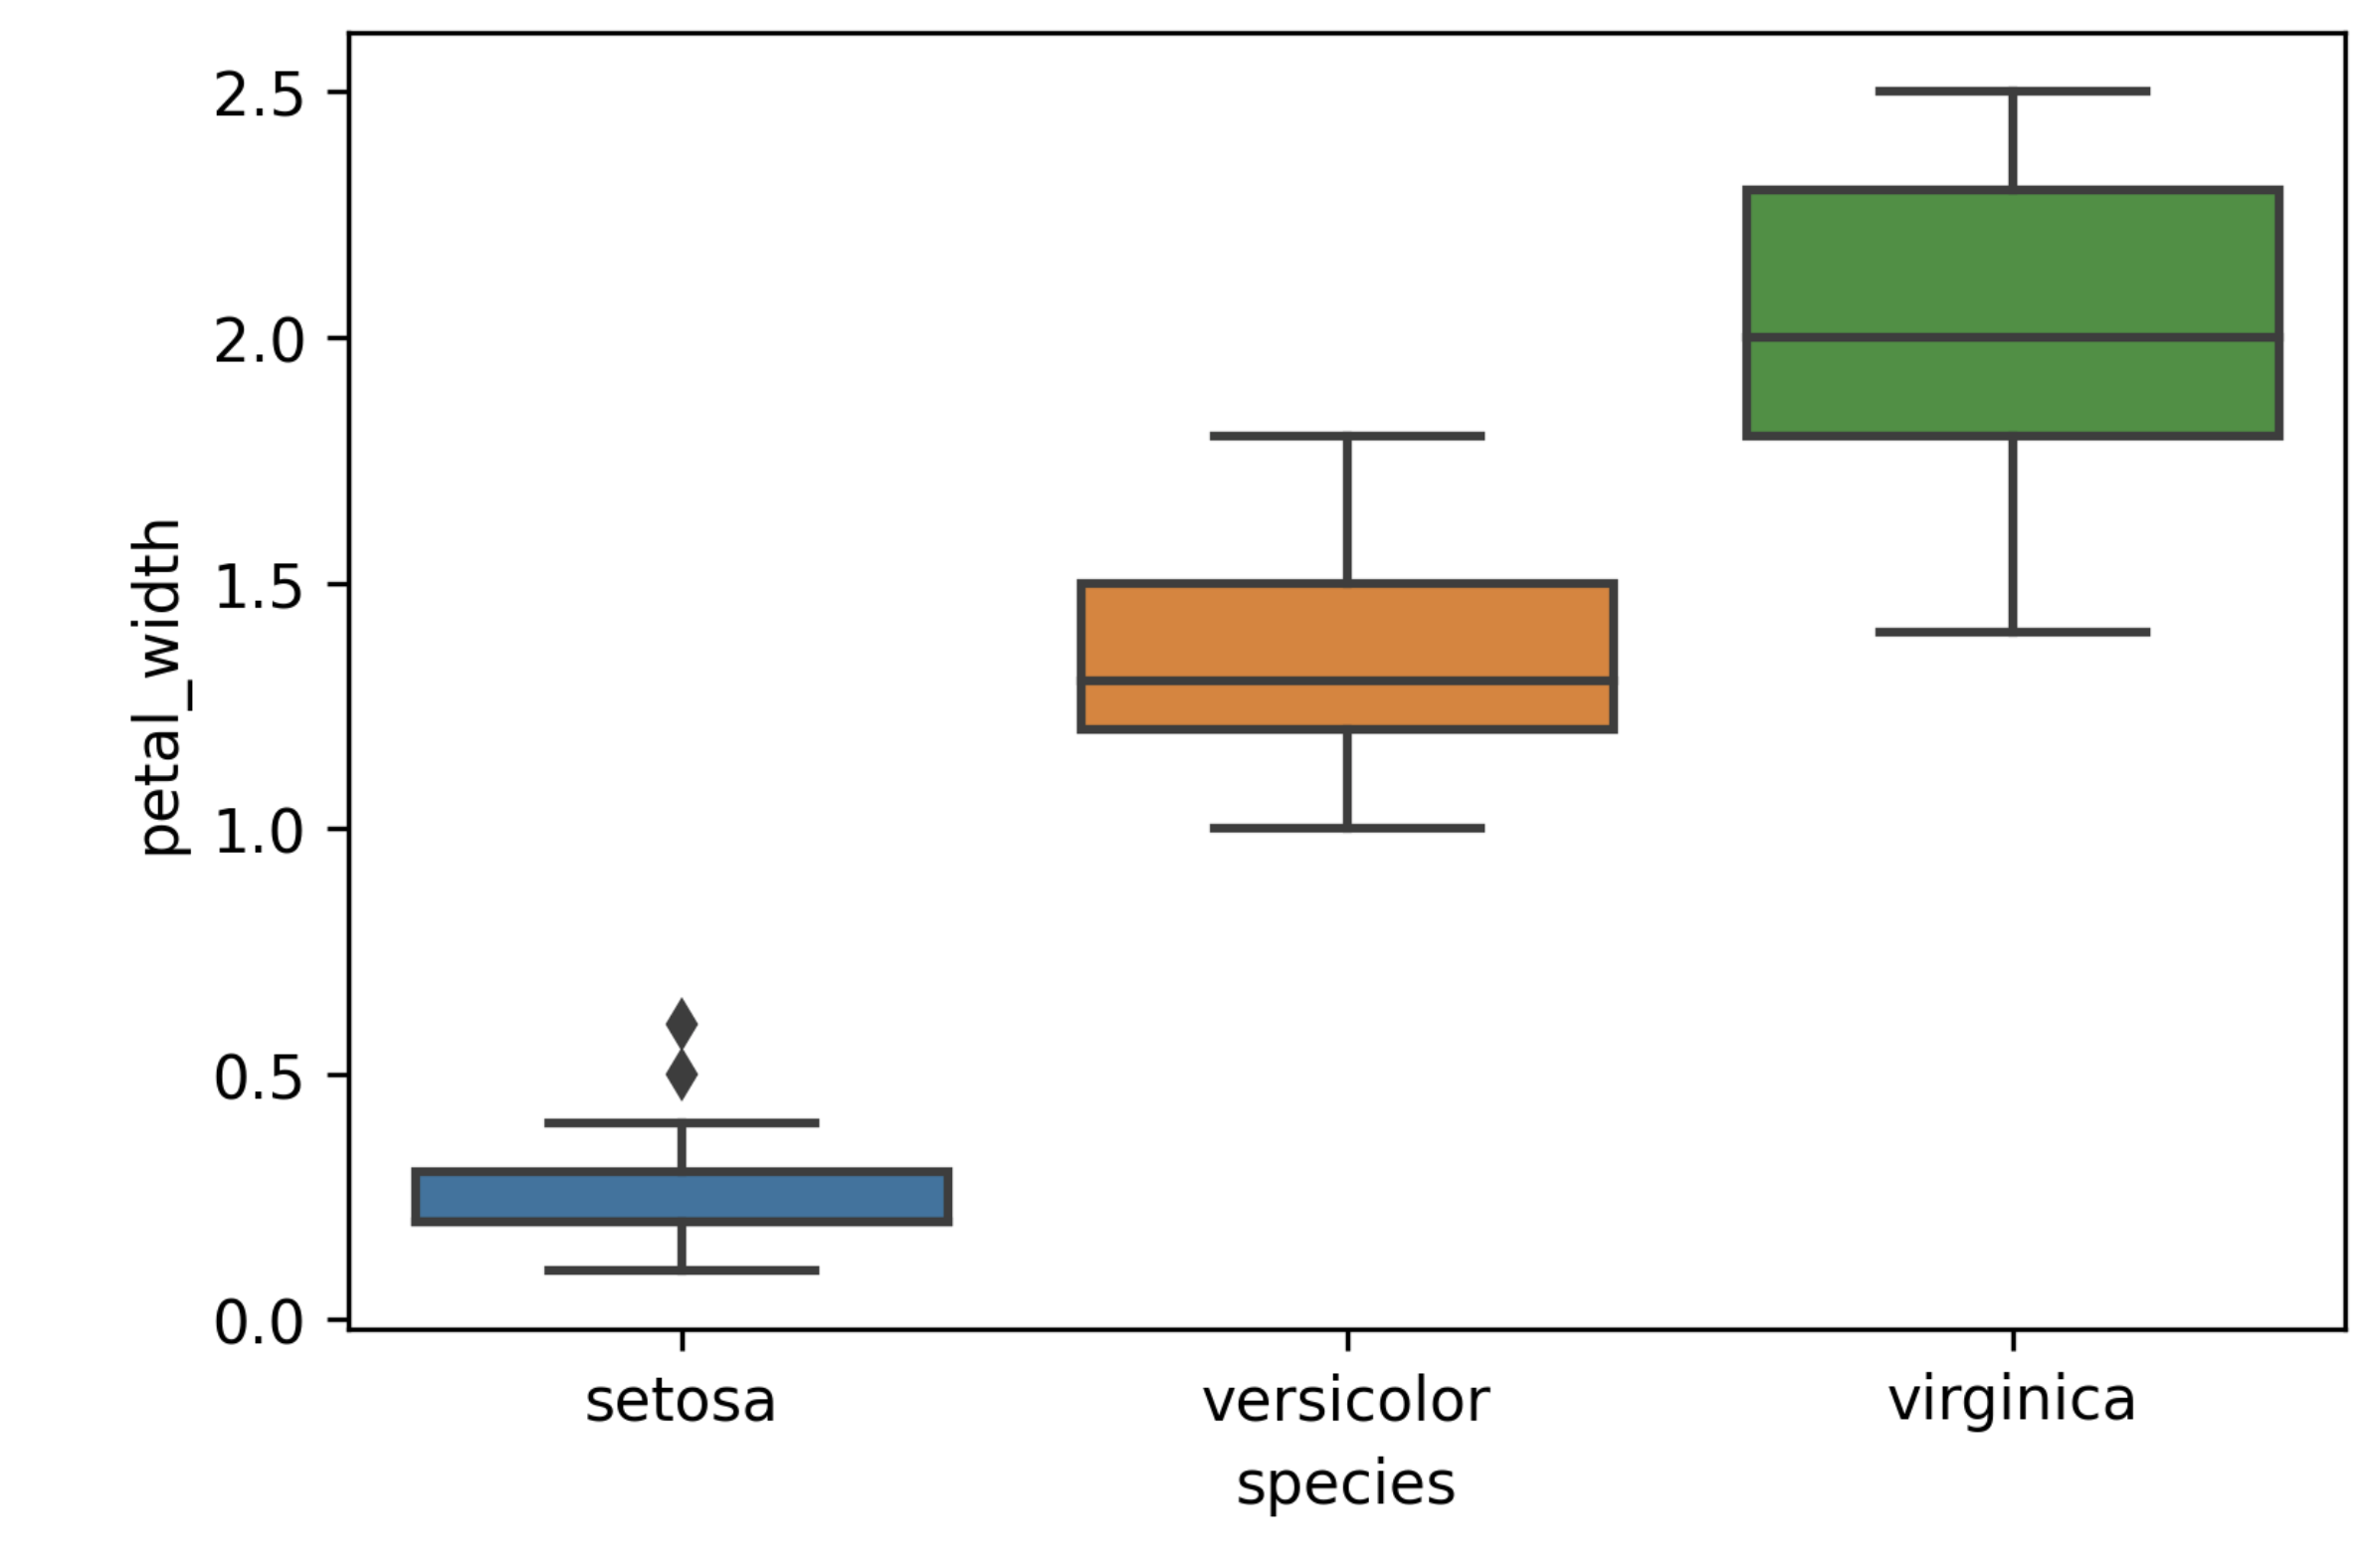
\includegraphics[width=0.7\textwidth]{figures/ssIM4.png}
    \caption{A boxplot showing petal width for different Iris species}
\end{figure}

We're still thinking quite small scale with this figure, so let's take a look at the data as a whole:

\begin{lstlisting}[language=Python]
    sns.pairplot(data=df, hue='species')
\end{lstlisting}

\begin{figure}[!h]
    \centering
    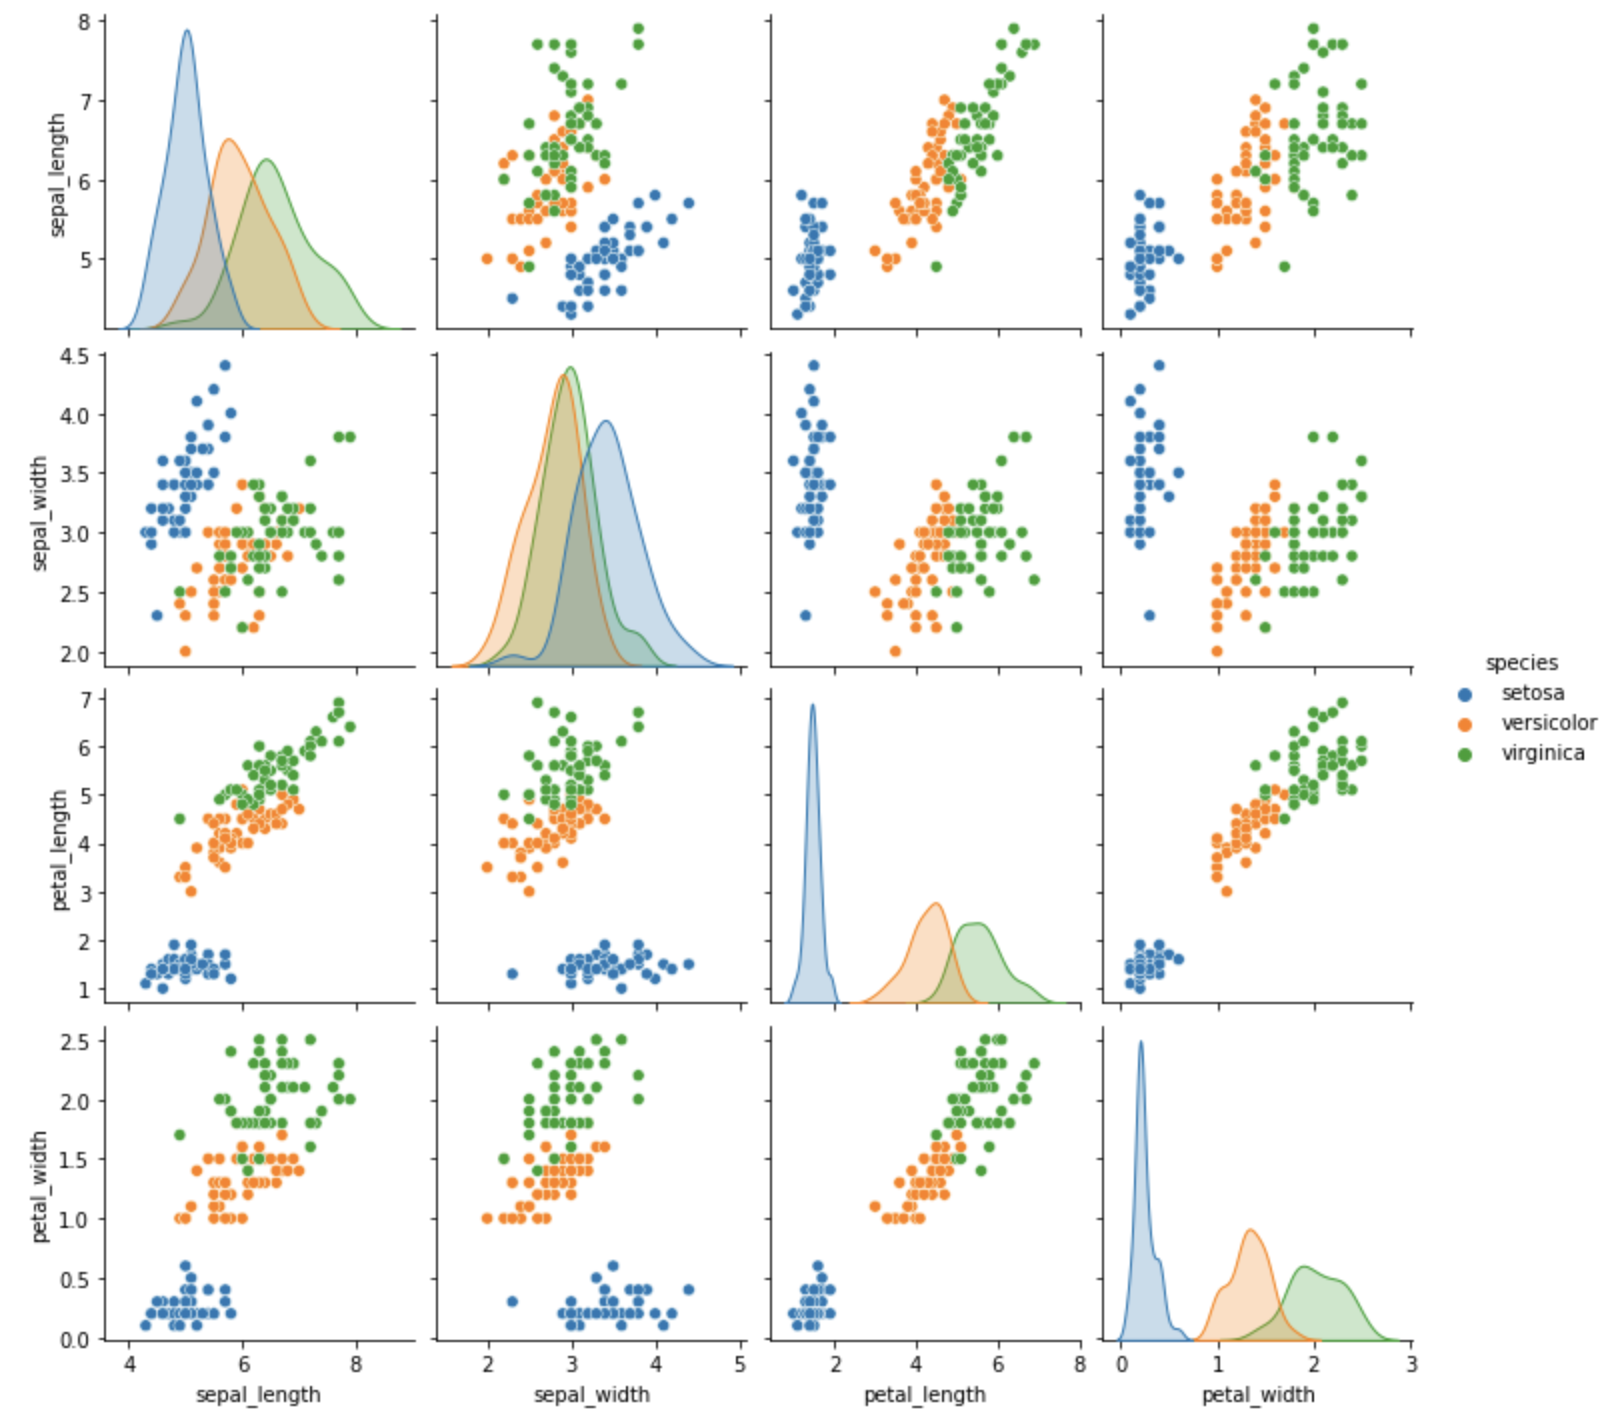
\includegraphics[width=0.9\textwidth]{figures/ssIM5.png}
    \caption{Pairplot of Iris data set features}
\end{figure}
\clearpage
\subsection{Statistical testing} 

Often, you will just want to know if "A is different from B", in Python this is fairly straight-forward. However, first you need to decide which test to do on your data to give the most appropriate results. Examples given here are heavily inspired by a great article which can be found here: \href{https://machinelearningmastery.com/statistical-hypothesis-tests-in-python-cheat-sheet/}{https://machinelearningmastery.com/statistical-hypothesis-tests-in-python-cheat-sheet/}

\subsubsection{Shapiro-Wilk Test}

The Shapiro-Wilk test will allow you to determine if your data fits a Normal distribution. Thus, our null hypothesis becomes "our data has a normal distribution". 

\begin{lstlisting}[language=Python]
    from scipy import stats
    setosa = df['species'] == 'setosa'
    setosa_sepal_length = df[setosa]['sepal_length']

    stats.shapiro(setosa_sepal_length)
\end{lstlisting}

Check the output of this command. It would suggest that the data are quite normally distributed so we can again visually check if we would like.
\begin{lstlisting}[language=Python]
    plt.hist(setosa_sepal_length)
\end{lstlisting}

\begin{figure}[!h]
    \centering
    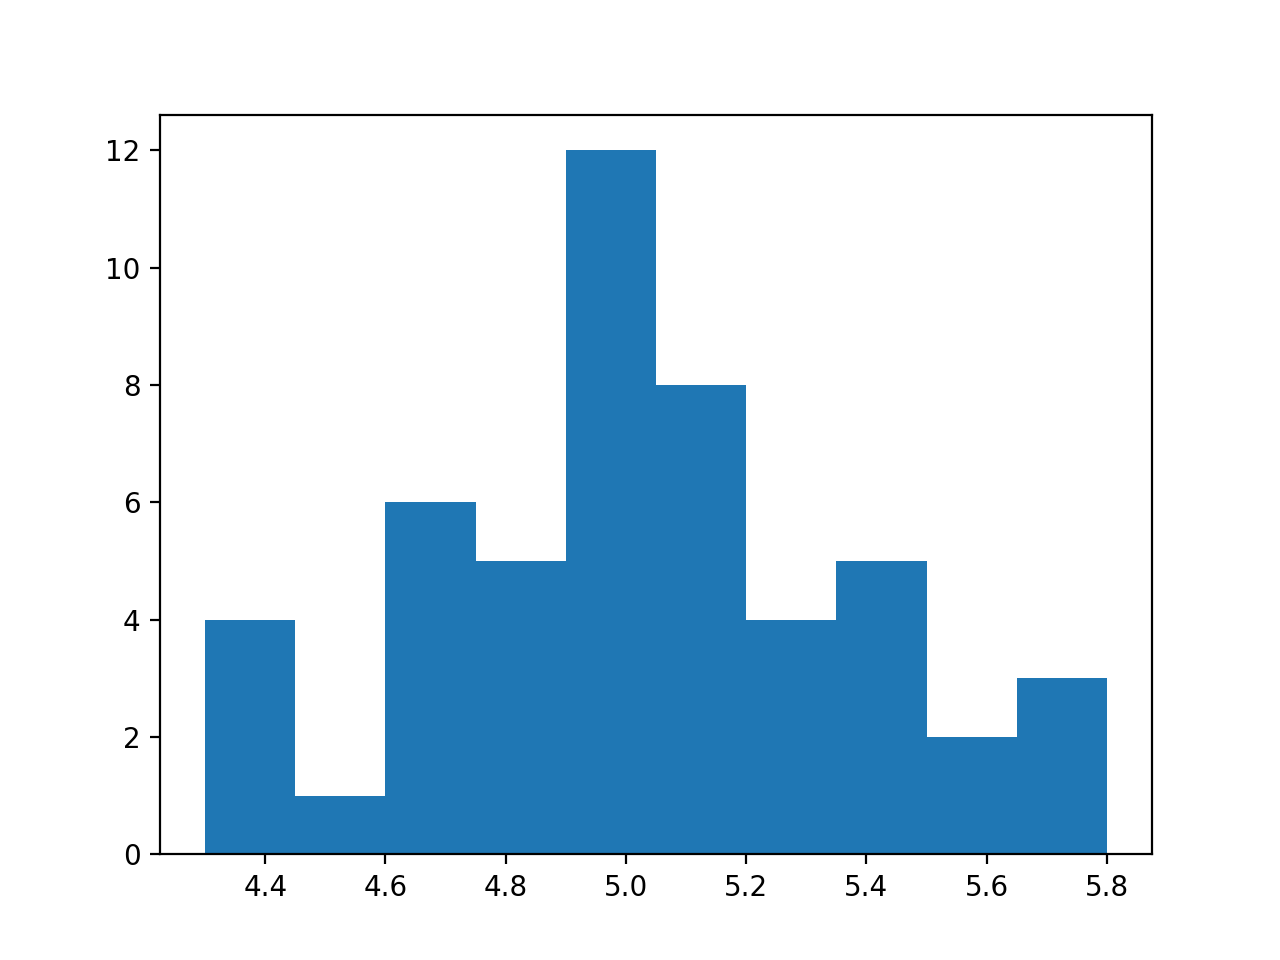
\includegraphics[width=0.4\textwidth]{figures/ssIM7.png}
    \caption{A quick histogram of Setosa's sepal length to verify distribution}
\end{figure}

Optionally, you can try and repeat this to check another species or another feature to see if it is also normally distributed.

\subsubsection{Student's t-Test}

Having evaluated our data and how 'normal' it is, we can proceed to choosing a statistical test. Most commonly used to biology, regardless of how correct or appropriate it is (\href{https://www.statisticsdonewrong.com}{https://www.statisticsdonewrong.com}, this is an excellent read, very funny and requires little maths experience), is the t-test. More specifically Student's t-test.  

Here, we perform a t-test between the sepal length of setosa and virginica plants.

\begin{lstlisting}[language=Python]
    from scipy import stats
    setosa = df['species'] == 'setosa'
    virginica = df['species'] == 'virginica'
    setosa_sepal_length = df[setosa]['sepal_length']
    virginica_sepal_length = df[virginica]['sepal_length']
    stats.ttest_ind(setosa_sepal_length, virginica_sepal_length, equal_var=False)
\end{lstlisting}

The first value returned is the t-statistic and the second, the commonly reported, p-value. 

\subsection{Building and testing a simple linear model}

For modelling, let's start simple. If we look at the previous plot we might be inclined to think that "petal\_length" and "petal\_width" have a linear relationship. So let us build a simple model using, 

\begin{equation}
    y = mx+b.
\end{equation}

Using another library this time, scipy, we can quite quickly find the ideal parameters for $m$ and $b$ in this model. We define our function "linear" to take an $x,m$ and $b$ and return a $y$ value. We specify our "xdata" and "ydata" to be "petal\_length" and "petal\_width", respectively. Then putting together with "curve\_fit" we get a "pars" list. This "pars" variable is just the $m$ and $b$ values for the model.  


\begin{lstlisting}[language=Python]
    from scipy.optimize import curve_fit

    def linear(x,m,b):
      return m*x+b
    
    xdata = df['petal_length']
    ydata = df['petal_width']
    
    pars, cov = curve_fit(f=linear, xdata=xdata, ydata=ydata)
\end{lstlisting}

Now, if we take those $m,b$ values we should be able to make a fairly decent prediction of "petal\_width" given the "petal\_length", if our assumption of linearity is apt. Remember, pars is a list of two values, so we need to pass it to our linear function correctly:

\begin{lstlisting}[language=Python]
    Y_pred = [ ]

    for x in xdata:
      Y_pred.append(linear(x, pars[0], pars[1]))
    
    plt.scatter(xdata, ydata, c='r')
    plt.plot(xdata, Y_pred)
    plt.xlabel('petal_length')
    plt.ylabel('petal_width')
\end{lstlisting}

\begin{figure}[!h]
    \centering
    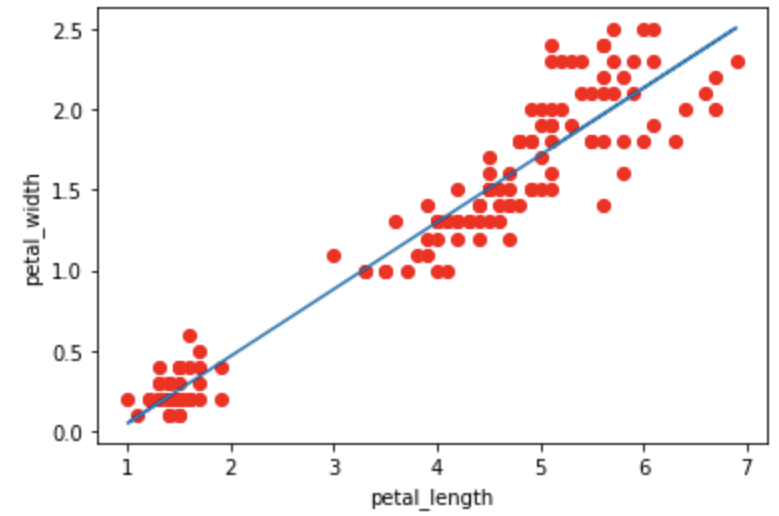
\includegraphics[width=0.7\textwidth]{figures/ssIM6.png}
    \caption{Plot testing our linear model with petal width and length measurements}
\end{figure}

This looks like a pretty good fit, but let's put some numbers behind it by calculating the $R^2$ value (calculated using \href{https://en.wikipedia.org/wiki/Coefficient_of_determination}{Coefficient of determination}):

\begin{lstlisting}[language=Python]
    residuals = ydata- linear(xdata, pars[0], pars[1])
    ss_res = np.sum(residuals**2)
    ss_tot = np.sum((ydata-np.mean(ydata))**2)
    r_squared = 1 - (ss_res / ss_tot)
    print(r_squared)
\end{lstlisting}


\clearpage
\appendix  
\section{Test solution}
\begin{lstlisting}[language=Python]
import matplotlib.pyplot as plt 
import numpy as np 

sin2_values = []
sin3_values = []
Xs = np.linspace(0,10, num=1000)

for x in Xs:
    sin2_values.append(np.sin(x)*2 )
    sin3_values.append(np.cbrt(np.sin(x)))

plt.plot(Xs, sin2_values, label="2 sin(x)")
plt.plot(Xs, sin3_values, label='cbrt(sin(x))')
plt.xlabel('x')
plt.ylabel('sin(x)')
plt.legend()
plt.grid()
\end{lstlisting}

\end{document}